\section{Kubernetes. Пространства имён. Метки. Переменные среды.}

\D{
    Namespace - подход для разделения рабочих пространств по проектам,
    командам, департаментам итд.
}

\begin{figure}[H]
	\centering
	\begin{minipage}[b]{0.8\textwidth}
		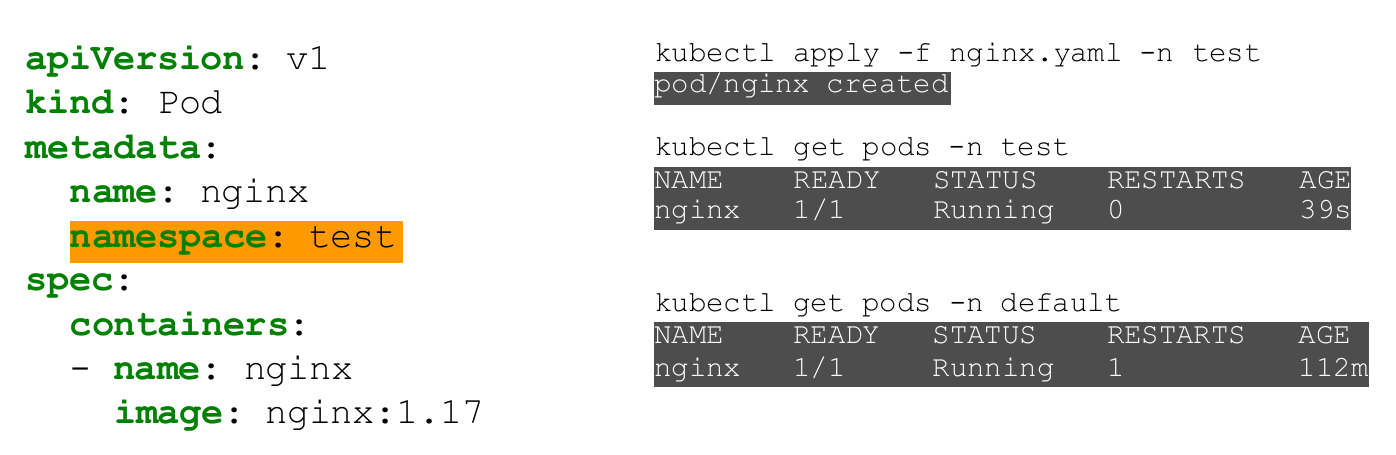
\includegraphics[width=\textwidth]{images/ns.png}
        \caption{Namespace}
	\end{minipage}
\end{figure}

\D{
    Labels - эффективный способ объединения объектов Kubernetes
    в логические группы для идентификации.

    Позволяют обращаться к пространству имен через ключевые значения.
}

Обращение по метке происходит через селектор.

\begin{figure}[H]
	\centering
	\begin{minipage}[b]{0.3\textwidth}
		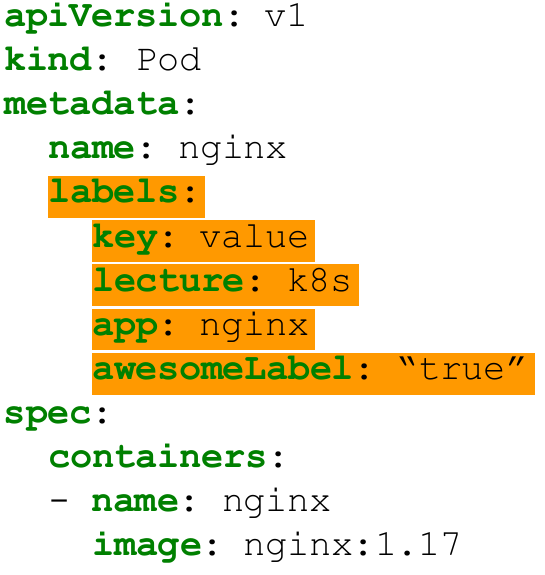
\includegraphics[width=\textwidth]{images/lab.png}
        \caption{Labels}
	\end{minipage}
\end{figure}

Переменные среды выставляются в конфиге пода через пары имя/значение
(выставляются в окружение пода).

Переменные плохо масштабируются и их сложно поддерживать.